
% \subsection{Phương pháp mã hóa phân tách khoảng cách tối đa}
% \label{CDC_des}

% Trước khi trình bày mô hình hệ thống, chúng tôi sẽ giới thiệu sơ qua cách thức hoạt động của điện toán phân tán dựa trên phương pháp mã hóa phân tách khoảng cách tối đa. Trong thời đại thông tin phát triển nhanh chóng, việc xử lý các tác vụ tính toán khối lượng lớn trên các thiết bị có thể gặp khó khăn, đặc biệt là đối với các thiết bị có tải công việc quá cao như các phương tiện giao thông. Với yêu cầu về kích thước nhỏ gọn, tiêu thụ năng lượng thấp và thời gian xử lý giới hạn, học tăng cường phân tán cho phép các phương tiện xử lý các nhiệm vụ tính toán lớn thông qua việc phân chia công việc. Nhiều phương tiện dịch vụ có thể thực hiện xử lý máy cục bộ dựa trên nhiệm vụ con được chỉ định từ các nhiệm vụ chính và truyền kết quả tính toán trở lại cho các nhiệm vụ chính của chúng để hoàn thành các nhiệm vụ lớn hơn. Tuy nhiên, hiệu suất của các hệ thống giảm tải lớn có thể bị ảnh hưởng đáng kể bởi các hạn chế như sự phân tán của các phương tiện dịch vụ, thời gian xử lý cục bộ vượt quá thời gian kết nối hoặc sự chậm trễ trong việc hoàn thành tính toán của các phương tiện dịch vụ so với nhau.

% Để giải quyết vấn đề này, một giải pháp hiệu quả đã được đề xuất bằng cách sử dụng kỹ thuật mã hóa để tạo ra một dự phòng thuận tiện cho việc tính toán. Ý tưởng cốt lõi của giải pháp này là mã hóa dữ liệu của nhiệm vụ chính vào các nhiệm vụ con tính toán của các phương tiện dịch vụ, sau đó chỉ yêu cầu các phương tiện dịch vụ trả về kết quả tính toán từ một tập hợp con nhanh nhất của chúng để giải mã và hoàn thành nhiệm vụ chính của mình. Do đó, thời gian xử lý của nhiệm vụ chính phụ thuộc vào tập hợp con nhanh nhất của các phương tiện dịch vụ hoàn thành nhiệm vụ phụ. Ngưỡng tối thiểu của số lượng phương tiện dịch vụ được lựa chọn dựa trên thiết kế mã hóa và yêu cầu của nhiệm vụ con.

% Hình.\ref{fig:MDS} minh họa một ví dụ về học tăng cường mã hóa trong hệ thống với một phương tiện chính và ba phương tiện dịch vụ $(n = 3)$. Phương tiện chính cần tính toán một phép nhân ma trận với một vector $(y = Ax)$ sử dụng Mã Hóa Tối Đa Khoảng Cách $(n = 3, m = 2)$.

% \textbf{Mã hóa và phân chia nhiệm vụ:} Phương tiện chính tách ma trận $\mathbf{A}$ trong không gian $\mathbb{R}^{r \times c}$ thành hai ma trận bằng nhau: $\mathbf{A_1}$ trong không gian $\mathbb{R}^{\frac{r}{2} \times c}$ và $\mathbf{A_2}$ trong không gian $\mathbb{R}^{\frac{r}{2} \times c}$. Sau đó, phương tiện chính gửi ma trận $\mathbf{A_1}$ cho phương tiện dịch vụ 1, ma trận $\mathbf{A_2}$ cho phương tiện dịch vụ 2, và ma trận $\mathbf{A_1}+ \mathbf{A_2}$ đến phương tiện dịch vụ 3 đồng thời truyền vector $x$ cho tất cả các phương tiện dịch vụ.

% \textbf{Nhận kết quả và giải mã:} Khi các phương tiện dịch vụ nhận nhiệm vụ con của mình, chúng tính toán đồng thời. Kết quả tính toán của các xe dịch vụ bao gồm $y_1 = A_1x$, $y_2 = A_2x$ và $y_3 = (A_1 + A_2)x$ tương ứng. Ngay sau khi tính toán hoàn tất, kết quả này được trả về cho phương tiện nhiệm vụ. Phương tiện nhiệm vụ có thể đạt được kết quả mong muốn $y = Ax$ miễn là nó nhận được bất kỳ hai kết quả tính toán từ các phương tiện dịch vụ, đó là ngưỡng của hệ thống. Ví dụ, trong Hình~\ref{fig:MDS}, nếu phương tiện dịch vụ 1 là phương tiện dịch vụ cuối cùng hoàn thành tính toán nhiệm vụ con, phương tiện nhiệm vụ có thể thu thập kết quả đầu ra mong muốn từ xe dịch vụ 2 và 3. Sau đó, phương tiện nhiệm vụ giải mã kết quả $y = (y_3 - y_2; y_2) = (A_1x; A_2x) = Ax$.


% \begin{figure}[h]
% \centering
% \begin{subfigure}{0.86\linewidth}
% 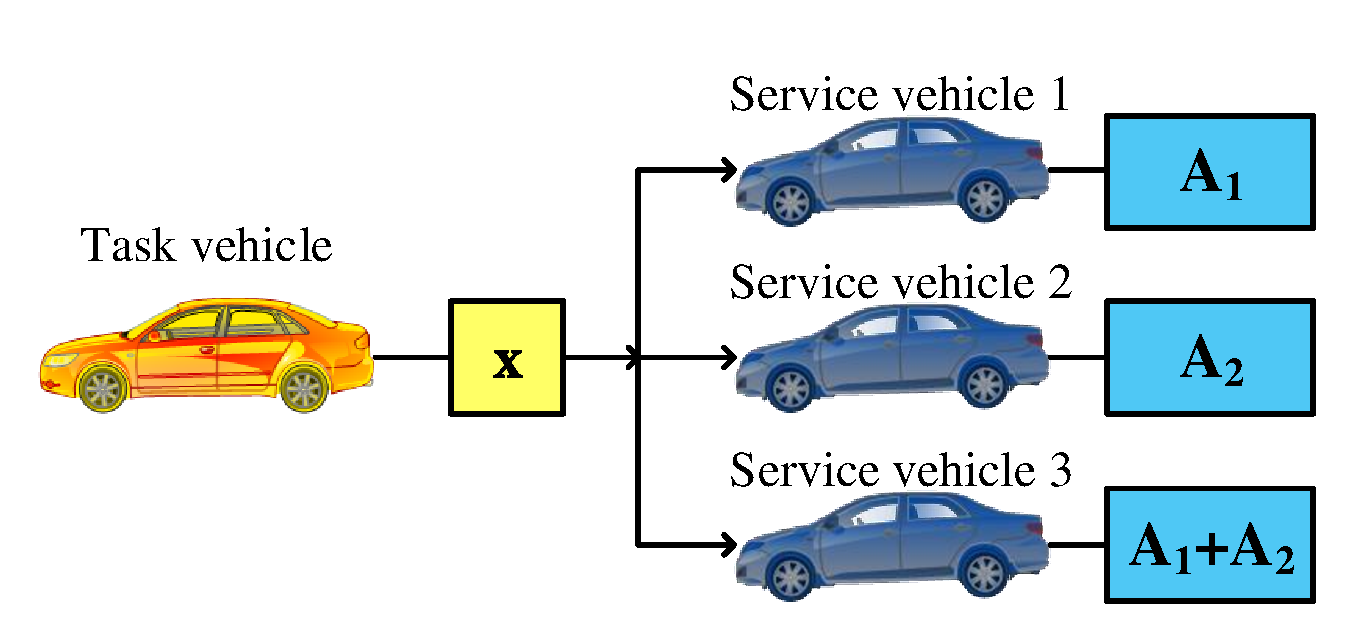
\includegraphics[width=\linewidth]{Images/MDS_example_part_a.pdf}
% \caption{Mã hóa và phân chia nhiệm vụ}
% \end{subfigure}

% \medskip
% \begin{subfigure}[b]{1.0\linewidth}
% 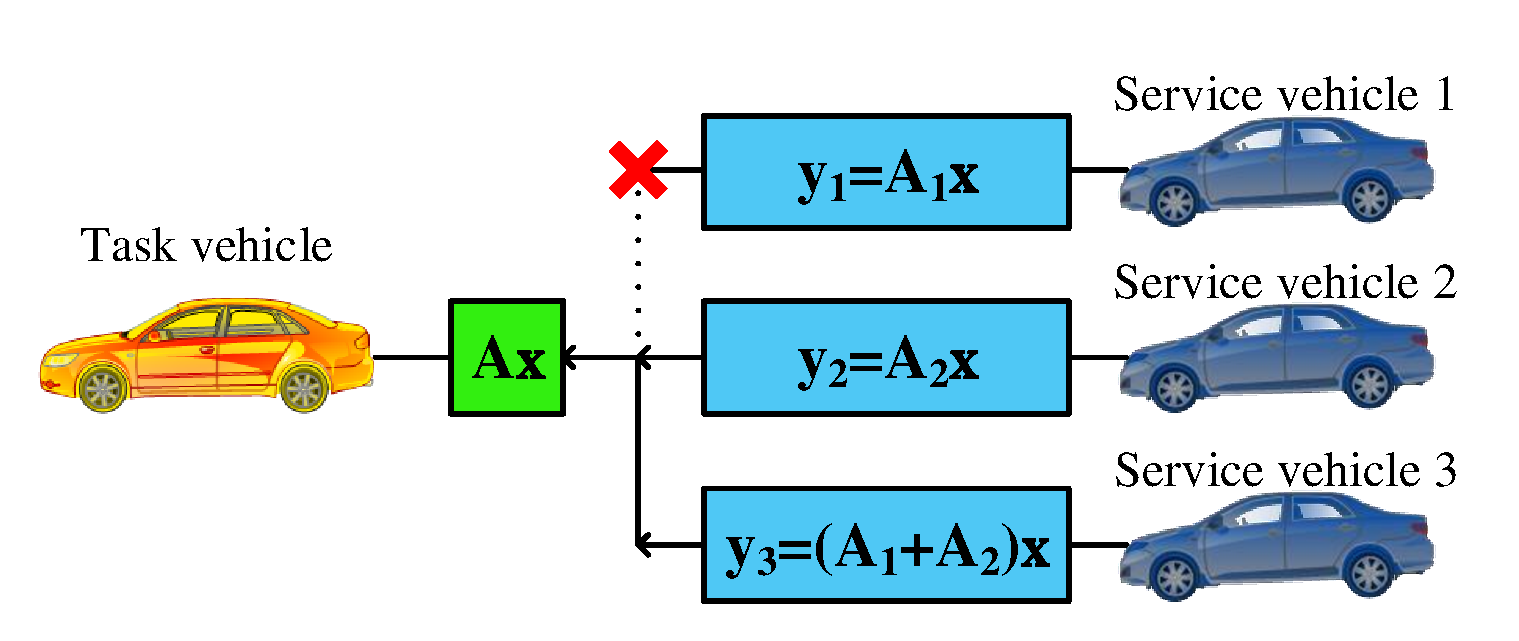
\includegraphics[width=\linewidth]{Images/MDS_example_part_b.pdf}
% \caption{Nhận kết quả và giải mã}
% \end{subfigure}

% \caption{Mã hóa máy học sử dụng mã hóa MDS}
% \label{fig:MDS}
% \end{figure}

% \subsection{Mô hình hệ thống}
% \label{model}
% Như đã trình bày trong chương giới thiệu, tôi sẽ xem xét hệ thông điện toán phân tán gồm các xe tự hành được trang bị DFRC. Trong phần này chúng ta sẽ cùng xem xét rõ mô hình hệ thống và cách thức hoạt động của hệ thống này. 

% \subsubsection{Mô hình vật lý hệ thống}
% \begin{figure}[h]
%     \centering/
%     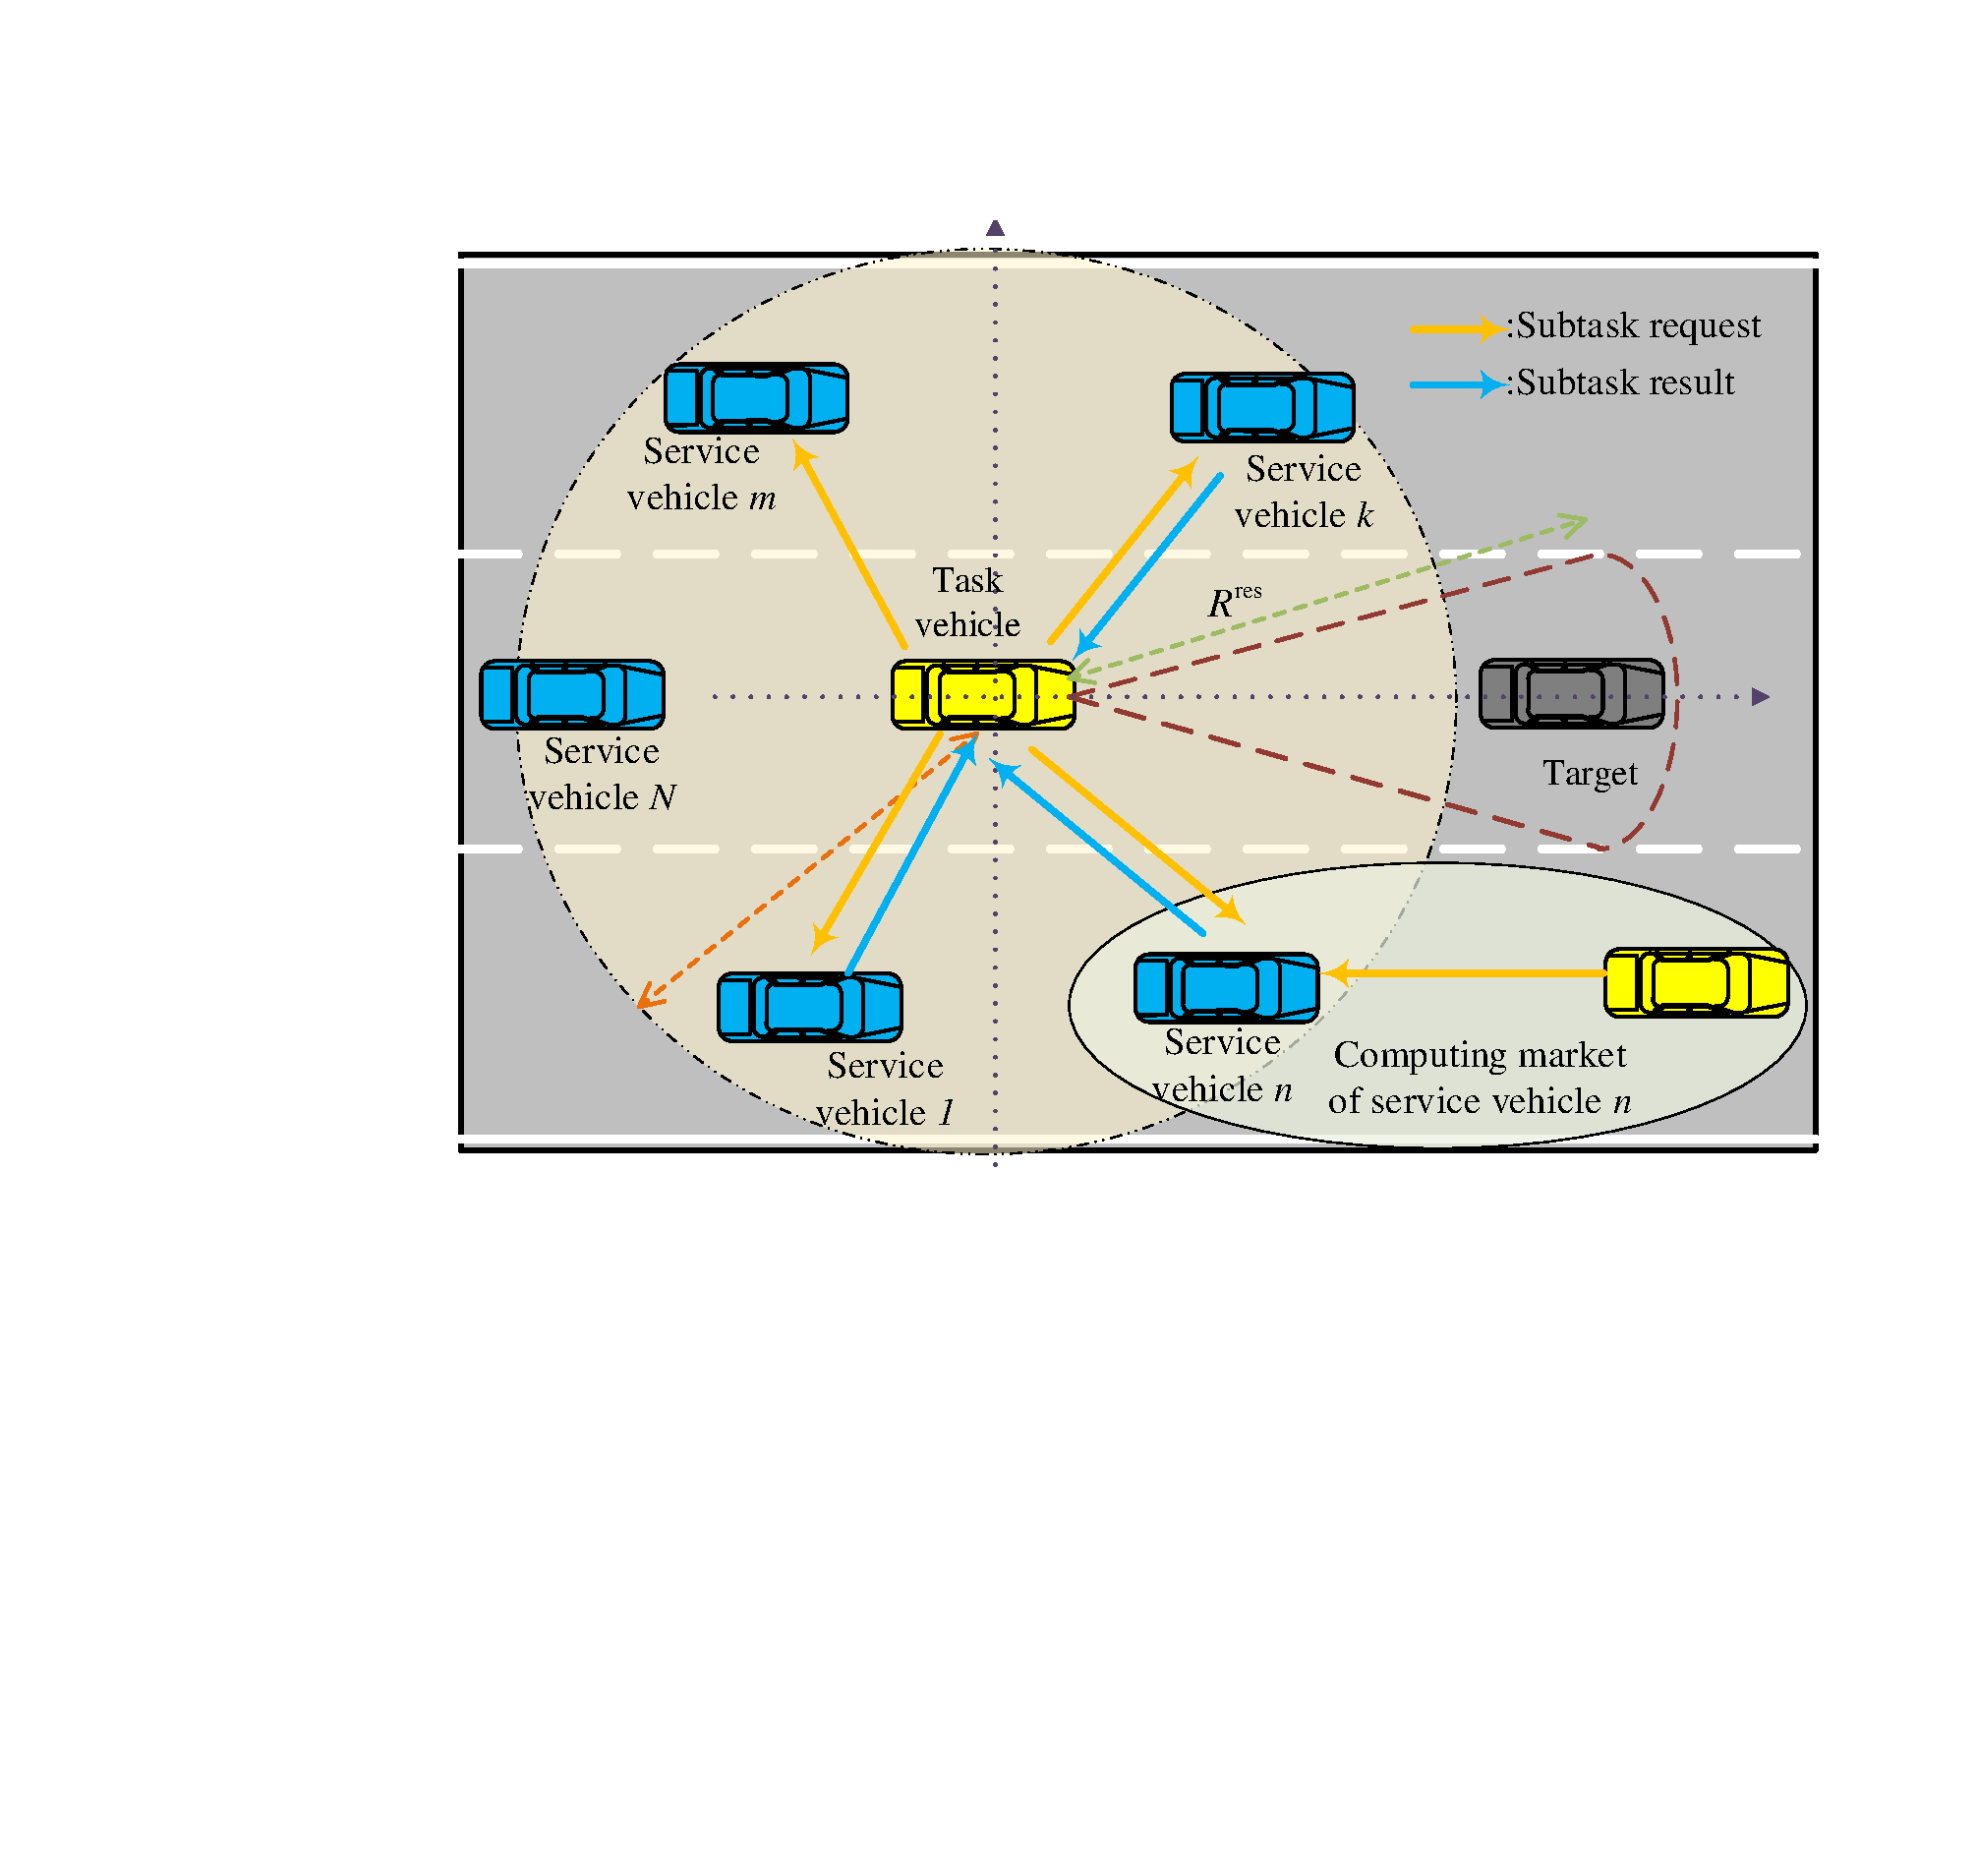
\includegraphics[width=1.0\textwidth]{Images/Model_SYS.pdf}
%     \caption{Mô hình hệ thống.}
%     \label{fig:systemmodel}
% \end{figure}

% Hình ~\ref{fig:systemmodel} cho ta thấy cái nhìn tổng quan về hệ thống. Nhằm đơn giản hóa hệ thống sẽ bao gồm 1 xe khách hàng đang tự hoạt động thực hiện các nhiệm vụ như giữ làm, giữ khoảng cách an toàn với xe mục tiêu,... và $N$ xe dịch vụ các xe này có nhiệm vụ giảm tải cho xe khách hàng. Các xe dịch vụ này có khả năng cung cấp các dịch vụ điện toán để có khả năng giảm tải cho xe khác hàng. Xét tại một thời điểm bất kì tôi giả sử rằng luôn có một tập hợp gồm $N$ xe dịch vụ trong vùng phủ sóng cả xe khách hàng. Xem xét mô hình thực tế do tính cơ động của các xe số lượng xe dịch vụ $N$ luôn luôn thay đổi theo thời gian. Một khía cạnh khác cần được xem xet đó là băng thông và không gian hoạt động, nhằm đảm bảo cho cả hệ thống lớn hoạt động tối ưu số lượng xe phục vụ cho xe khách hàng sẽ bị giới hạn $N<N_{max}$ trong đó $N_{max}$ là số lượng xe dịch vụ tối đa có sẵn xung quanh xe khách hàng. Khi mồ hình hóa hệ thống tôi nhận thấy còn tồn tại một vấn đề nữa đối với giá trị $N$, trong thực tế khi lưu thông trên đường các xe tương tác với nhau trong không gian dẫn đến mật độ xe không phải là đại lượng mang tính ngẫu nhiên. Trong mô hình hệ thống chúng ta phải xem xét số xe dịch vụ $N$ trong phạm vi kết nối của xe khách hàng là thông số không ngẫu nhiên. Để mô hình hóa điều này tôi đề xuất sử dụng quá trình Markov.


% \textbf{Quá trình Markov:} Markov chain \cite{markov}, còn được gọi là quá trình Markov, là một mô hình toán học được sử dụng để mô tả sự di chuyển ngẫu nhiên giữa các trạng thái khác nhau trong hệ thống. Nó được đặt tên theo nhà toán học người Nga Andrei Markov. Một quá trình Markov được xác định bởi tập hợp các trạng thái khả dĩ và các xác suất chuyển từ một trạng thái sang trạng thái khác. Mỗi trạng thái có một xác suất chuyển riêng, đồng thời, xác suất chuyển chỉ phụ thuộc vào trạng thái hiện tại và không phụ thuộc vào lịch sử di chuyển trước đó. Điều này được gọi là tính chất Markov, tức là tính không gian của quá trình chỉ phụ thuộc vào trạng thái hiện tại.

% \begin{figure}[h]
%             \centering 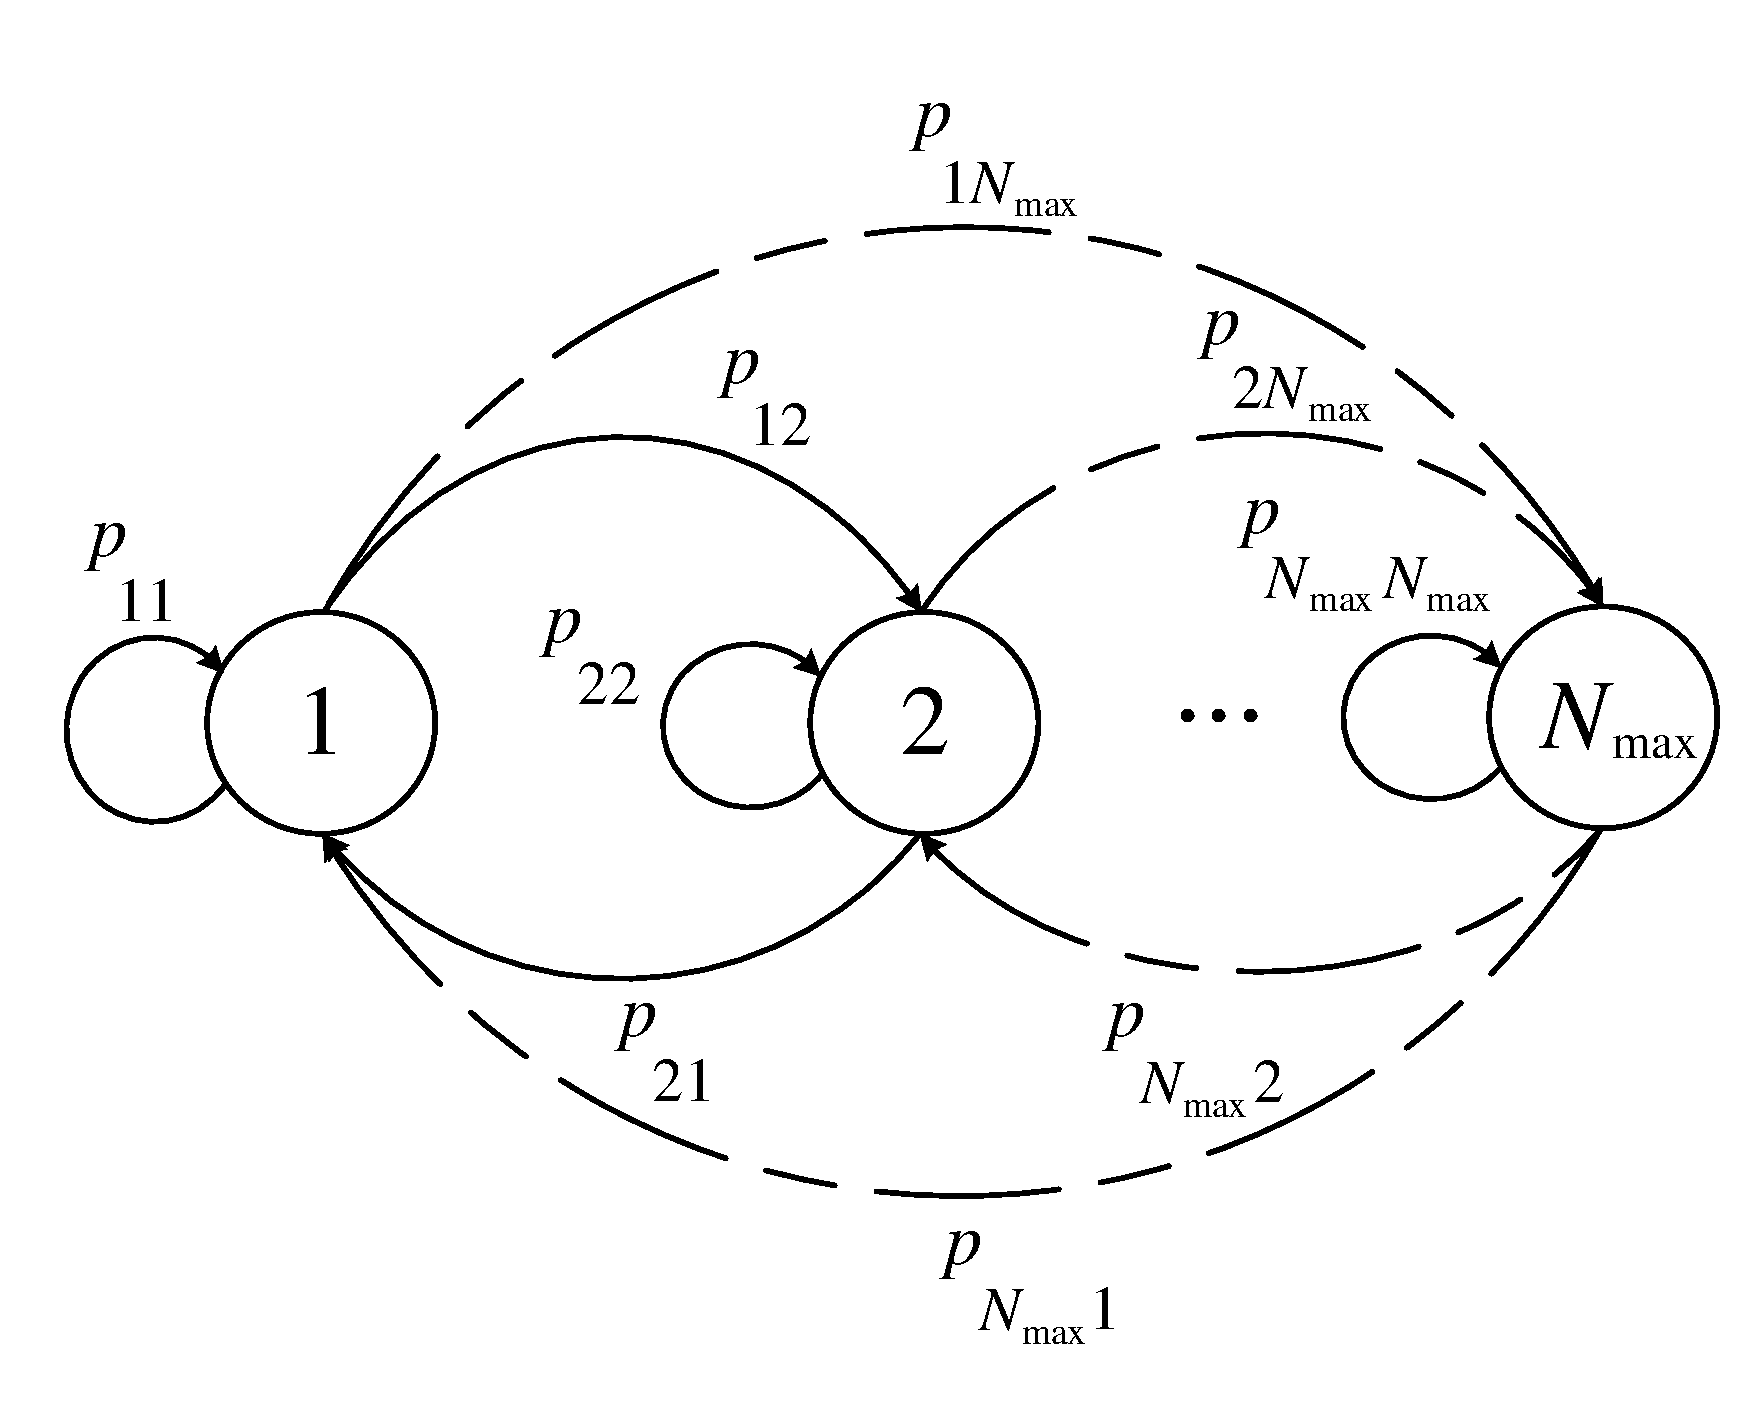
\includegraphics[width=1.0\textwidth]{Images/Sodotrangthai.pdf}
%             \caption{Sở đồ chuyển đổi trang thái số lượng xe dịch vụ $N$.}
%             \label{fig:trans_state}
% \end{figure}

% Quá trình Markov có thể được sử dụng để mô hình hóa và dự đoán các quá trình ngẫu nhiên, chẳng hạn như việc dự đoán thời tiết, lưu lượng giao thông, hành vi tài chính, và nhiều ứng dụng khác. Nó cũng được ứng dụng trong lĩnh vực kỹ thuật, khoa học dữ liệu, và trí tuệ nhân tạo để phân tích và dự đoán các hệ thống phức tạp. Cụ thể với giá trị $N\in [1,2,...,N_{max}]$ là trạng thái số lượng xe dịch vụ có thể kết nối với xe khách hàng, các trạng thái này chuyển đổi tuân theo quá trình Markov cách thức hoạt động được mô tả trong hình~\ref{fig:trans_state}

% Xác suất thay đổi trạng thái có thể biểu thị bằng mà trận $P$ như sau:
% \begin{equation}
%              \label{ep:P_matrix}  
%              \mathbf{P} = [p_{ij}]_{N_{\rm{max}} \times N_{\rm{max}}}=
%              \begin{bmatrix}
%                  p_{11} & \cdots  &p_{1N_{\rm{max}}}\\
%                  \vdots &\ddots & \vdots\\
%                  p_{N_{\rm{max}}1} & \cdots  &p_{N_{\rm{max}}N_{\rm{max}}}
%             \end{bmatrix},
% \end{equation}
% trong đó $p_{ij} = P(N_{t+1} = j|N_t = i)$ đề cập đến xác suất rằng số lượng phương tiện dịch vụ có sẵn thay đổi từ $i$ đến $j$ từ thời gian $t$ đến $t + 1$.

% Cuối cùng, tôi giả định rằng trong quá trình di chuyển của các phương tiện có một hệ tọa độ trong đó xe khách hàng là cơ sở của hệ tọa độ. Khi đó, thông tin trạng thái của xe dịch vụ $n\in N$ cần thiết cho quyết định giảm tải của xe nhiệm vụ có thể được thể hiện bằng:
% \begin{equation}
% (x_n, v_{x_n}, y_n, v_{y_n}, f_n, c_n),
% \end{equation}
% Trong đó $x_n, v_{x_n} , y_n$ và $v_{y_n}$ là vị trí và vận tốc của xe dịch vụ $n$ dọc theo trục $x$ và $y$ tương ứng, $f_n$ đại diện cho tài nguyên CPU khả dụng của xe dịch vụ và $c_n$ đại diện cho giá trị tính toán trên một đơn vị thời gian. Chúng tôi biểu thị $d_n= \sqrt{x_n^2 + y_n^2}$ là khoảng cách giữa xe khách hàng và xe dịch vụ $n$. 

% \subsubsection{Khả năng kết nối}

% Như đã đề cập ở muc~\ref{sec:1.2} xe được trang bị DFRC dùng chung nguồn năng lượng cho các tác vụ. Điều này gây ảnh hưởng tới phạm vi hoạt động của radar. Trong phần này tôi trình bày khả năng kết nối và tìm ra công thức phạm vi hoạt động của radar.

% Xe khách hàng có nhiệm vụ điều chỉnh đường đi, phát hiện và theo dõi các xe khác, và công việc này được hỗ trợ bởi DFRC. Xe khách hàng sử dụng chức năng giao tiếp để mã hóa và truyền nhiệm vụ cho các xe dịch vụ, nhằm giảm tải công việc. Việc phát hiện và theo dõi các xe khác được thực hiện bằng cách phát tín hiệu đến mục tiêu và sau đó xác định các thông số như tọa độ và vận tốc dựa trên tín hiệu trả về từ các xe khác. Trong quá trình này, có hai đại lượng quan trọng là độ phân giải khoảng cách (range resolution), xác định khoảng cách tối thiểu giữa hai mục tiêu mà radar có thể phân biệt được, và phạm vi radar, là khoảng cách tối đa mà radar có thể phát hiện các đối tượng. Để đơn giản hóa mô hình, tôi giả sử rằng có duy nhất một mục tiêu ở trong phạm vi hoạt động của radar (như trong hình~\ref{fig:systemmodel}). Như vậy chỉ có thể tồn tại tối đa một mục tiêu duy nhất trong phạm vi hoạt động của radar. Do đó tôi sử dụng phạm vi của radar thay vì độ phân giải khoảng cách làm thước đo hiệu suất của chức năng radar. Lưu ý rằng chức năng của radar có thể sử dụng các tín hiệu của chức năng giao tiếp cho tác vụ phát hiện và theo dõi mục tiêu. Tuy nhiên, khi sử dụng phương pháp này, hiệu suất chức năng của radar không ổn định vì phục thuộc nhiều bởi các lại dữ liệu truyền và thông tin của chức năng liên lạc~\cite{luong2021radio}.

% Xem xét DFRC, đối với radar thông thường sẽ dùng sang liên tục được điều chế tần số, DFRC chức năng radar và chức giao tiếp thông tin sử dụng chung nguồn điện. Kí hiệu $P^{\rm{tx,rad}}$ là công suất phát của chức năng radar. Vì $P^{\rm{tx,com}}=\mu P^{\max}$ được sử dụng cho chức năng giao tiếp, do đó $P^{\rm{tx,rad}}=P^{\max}\left(1-\mu \right)$ được sử dụng cho chức năng radar. Từ đó chúng ta có thể tính được công suất của tín hiệu dội lại tại máy thu của radar là~\cite{chu2020interference}:
% \begin{align}\label{rec_power}
% P^{\rm{rx,rad}}&=\\
% &\underbrace{ \frac{ P^{\max}\left(1-\mu \right) G^{\rm{tx,rad}} \sigma_c}{4 \pi \left(R^{\rm{range}}\right)^4  }}_{\text{Mật độ năng lượng phản xạ}} \times \underbrace{ \frac{\left(\lambda^{\rm{rad}}\right)^2G^{\rm{rx,rad}}}{ 4 \pi } }_{\text{Diện tích anten thu hiệu quả}}, \notag
% \end{align}
% Trong đó $G^{\rm{tx,rad}}$ và $G^{\rm{rx,rad}}$ gain của anten của máy phát và máy thu của radar, $\lambda^{\rm{rad}}=c/f^{{\rm{rad}}}$ với $f^{{\rm{rad}}}$ là tần số hoạt động của radar và $\sigma_c$ là tiết diện của radar tính bằng $m^2$. Tiết diện của anten tỉ lệ thuận với kích thước và hình dạng của mục tiêu. Ví dụ: $\sigma_c= 120m^2$ đối với ô tô có kích cỡ trung bình và $\sigma_c=60m^2$ đối với ô tô có kích thước nhỏ. Để đảm bảo phát hiện mục tiêu, tín hiệu phản xạ phải lớn hơn mức tối thiểu của tín hiệu mà xe khách hàng có thể phát hiện được. Như vậy, phạm vi tối đa của radar có thể xác định được được định nghĩa là giá trị mà tại đó $P^{\rm{rx,rad}}=P^{\rm{rx,rad}}_{\rm{min}}$. Bằng cách thay $P^{\rm{rx,rad}}=P^{\rm{rx,rad}}_{\rm{min}}$ vào công thức ~\eqref{rec_power} chúng ta có thể tính được $R^{\rm{range}}$ là tầm hoạt động tối đa của radar trên xe khách hàng:
% \begin{equation}
%   \label{radar_range}    
%   R^{\rm{range}}=\left( \frac{\left(1-\mu\right)P^{\max} G^{\rm{tx,rad}}G^{\rm{rx,rad}} (\lambda^{\rm{rad}})^2 \sigma_c }{4\pi^2 P^{\rm{rx,rad}}_{\rm{min}}} \right)^{1/4}.
% \end{equation}
% Từ công thức trên dễ dàng thấy được $R^{\rm{range}}$ tỉ lệ thuận với $\left(1-\mu\right)P^{\max}$. Khi giảm $\mu$, $\left(1-\mu\right)P^{\max}$ tăng và từ đó $R^{\rm{range}}$ cũng tăng lên. Tuy nhiên, khi giảm $\mu$, công suất của chức năng giao tiếp sẽ giảm. Điều này dẫn đễn tăng thời gian giảm tải và tổng thời gian tính toán. Do đó, cần phải tối ưu hóa hệ số công suất $\mu$ để đảm bảo thời gian giảm tải và phạm vi của radar.

% \subsubsection{Quá trình xử lý tác vụ}
% Các xe dịch vụ được thiết lập có chức năng giảm tải tác vụ cho xe khách hàng với mục tiêu xử lý tác vụ một cách nhanh nhất. Quá trình xử lý được xem xét trong phần này và tôi sử dụng thời gian xử lý nhằm đánh giá hiệu quả của quá trình xử lý này. 

% \textbf{Tác vụ:} Nhằm mô hình hóa tác vụ, tôi sử dụng $L$ được tính bằng bit đại diện cho kích thước tác vụ mà xe khách hàng cần phải xử lý. Tác vụ phải được xử lý trong thời gian nhất định nhằm đảm bảo trải nghiệm của người dùng, tránh các tình trạng hệ thống hoạt động không hiệu quả dẫn đến các tính huống nguy hiểm có thể xảy ra với xe khách hàng và các xe khác lưu thông trên đường. Tôi đặt thời gian quy định này là $t^{req}$. Bằng cách áp dụng mã hóa MDS đã trình bày trong mục ~\ref{CDC_des}, tôi đặt ra cặp giá trị $(m,k)$. Đầu tiên từ tác vụ có kích thước $L$ bits được chia thành $k$ tác vụ cung có kích thước $L/k$ như nhau. Sau đó, tác vụ con này được mã hóa thành $m (1 \leq k \leq N)$ tác vụ con mã hóa. Lưu ý rằng các tác vụ con sau khi được mã hóa vẫn có kích thước $L/k$ bits. Cuối cùng xe khách hàng chọn $m$ trong số $N$ xe dịch vụ để thực hiện $m$ tác vụ đã được mã hóa.

% \textbf{Quá trình truyền tải và xủ lý:} Do xe khách hàng chọn $m$ xe dịch vụ nhằm thực hiện quá trình giảm tải, ta có thể dễ dàng thấy được tổng độ trễ của quá trình tính toán bao gồm thời gian truyền giảm tải, thời gian tính toán xử lý tác vụ và thời gian trả kết quả về.
% \begin{itemize}
%     \item Xem xét quá trình truyền tác vụ giảm tải: Tôi đặt $t^{\rm{off}}_n$ là thời gian của quá trình truyền tác vụ giảm tải đã được mã hóa đến xe dịch vụ $n$. Do chia sẻ nguồn năng lượng với tác vụ radar nên $P^{\rm{tx,com}}=\mu P^{\max}$ là công suất mà xe khách hàng dùng cho tác vụ giao tiếp. $t^{\rm{off}}_n$ được tính theo công thức:
%     \begin{equation}
%         t^{\rm{off}}_n= \frac{L}{kr_n},
%     \end{equation}
%     Trong đó $r_n$ là tốc độ truyền dữ liệu xe khách hàng đến xe dịch vụ $n$ được biểu diễn theo công thức:
%     \begin{equation}
%     r_n =  B_m\log_2\left(1 + \frac{ \mu P^{\max}G^{\rm{tx,com}}G^{\rm{rx,com}}_n\beta h_nd_n^{-\delta}}{\mathcal{I}+B_m\sigma^2}\right),
%     \label{data_rate_off}
%     \end{equation}
%     Trong đó $B_m=B/m$ là băng thông được phân bố cho kết nối giữa xe khách hàng và xe dịch vụ $n$, $\mathcal{I}$ biểu đạt sự can thiệp gây ra bởi việc chia sẻ cung phổng tần giữa xe khách hàng và các xe dịch vụ, $\sigma^2$ là phương sai nhiễu, $G^{\rm{tx,com}}$ và $G^{\rm{rx,com}}_n$ lần lượt là độ lợi anten phát của xe nhiệm vụ và độ lợi anten thu của xe dịch vụ $n$, $h_n$ là độ lợi kênh và $\beta_n=\left(\frac{c}{4\pi f_c}\right)^2$ với $f_c$ là tần số hoạt động của xe khách hàng và $c$ là vận tốc ánh sáng.
%     \item Quá trình xử lý tác vụ giảm tải: Sau khi nhận được các nhiệm vụ con được mã hóa từ xe khách hàng, các xe dịch vụ sử dụng tài nguyên máy tính của họ để thực hiện các nhiệm vụ xử lý nhằm giảm tải cho xe khách hàng. Tôi biểu thị $f_n$ là tài nguyên CPU có sẵn của xe dịch vụ n. Tài nguyên này thể hiên khả năng xử lý của xe dịch vụ. Trên thực tế các xe dịch vụ vẫn phải thực hiện các tác vụ của riêng mình, điều này dẫn đến tài nguyên CPU thực sự sử dụng cho tác vụ giảm tải có thể lớn hơn hoặc nhỏ hơn giá trị $f_n$. Tiếp theo chúng ta xem xét đến thời gian tính toán giảm tải của xe dịch vụ $n$. Thời gian này được tính theo công thức:
%     \begin{equation}
%     t_n^{\rm{comp}} = \frac{L}{f_nk}.
%     \end{equation}
%     Như đã đề cập $f_n$ có thể thay đổi vì cậy giá trị $t_n^{\rm{comp}}$ cũng sẽ thay đổi theo. Kế thừa chứng mình trong ~\cite{fix} ta có định lý sau về phân phối của $t_n^{\rm{comp}}$
%     \begin{theorem}
%     Sự phân bố thời gian tính toán $t_n^{\rm{comp}}$ có thể được biểu diễn bằng phân phối chuẩn như sau: 
%         \begin{equation}
%         \label{tcomp}
%             t_n^\mathrm{comp} = {\mathcal {N}}\left(\frac{L}{f_nk},\sigma^{2}_{t_n^{\rm{comp}}} \right),
%         \end{equation}
%     Trong đó $\frac{L}{f_nk}$ và $\sigma^{2}_{t_n^{\rm{comp}}}$ là giá trị trung bình và phương sai của phân bổ. Điều này được chứng minh trong phần Phục lục.
%     \end{theorem}
%     \item Cuối cùng chúng ta xem xét quá trình truyền tải kết quả từ xe dịch vụ tới xe khách hàng. Về cơ bản quá trình này có độ trễ không đáng kể so với quá trình tính toán hay quá trình truyền tải đến xe dịch vụ vì liên kết giao tiếp giữa các xe đã được hình thành.
% \end{itemize}

% Tổng kết lại tổng thời gian cho toàn bộ quá trình giảm tải giữa xe khách hàng và xe dịch vụ sẽ được tình theo công thức:  
% \begin{equation}
%     t_n = t_n^\mathrm{off} + t_n^\mathrm{comp}.
%     \label{d_total}
% \end{equation}
% Tuy nhiên độ trễ của hệ thống phải xem xét tất quả các quá trình xử lý đối với $N$ xe dịch vụ. Do đó tổng thời gian của quá trình giảm tải sẽ là:
% \begin{equation}
%     t^{\rm{over}} = \min_{1\leq k \leq m}\{ t_k^{\rm{over}}\}.
%     \label{d_total}
% \end{equation}

% Khi xem xét cụ thể quá trình kết nối tôi nhận thấy rằng tính cơ động của xe gây ra một vấn đề rằng sẽ có trường hợp các xe đang trong quá trình xử lý sẽ thoát khỏi vùng phủ của chức năng giao tiếp của DFRC. Dẫn đến vấn đề mất kết nối đây là một nguyên do dẫn đến quá trình xử lý bị ảnh hưởng trầm trong. Nhằm khác phục vấn đề này chúng ta phải ràng buộc $t_n \leq \xi_n$. Trong đó $t_n$ là thời gian xử lý và $\xi_n$ là thời gian mà xe dịch vụ thoát khỏi bán kình phủ. Giá trị $\xi_n$ được tính theo công thức:
% \begin{equation}\label{connection_time}
% \xi_n =\frac{R^{\rm{cov}}}{|v_{x_n} - v_t|} - \frac{x_n-x_t}{v_{x_n} - v_t},
% \end{equation}
% Trong công thức trên, không mất tính tổng quát tôi giả sử rằng các xe dịch vụ chỉ chuyển động theo trục $x$. Khi đó $R^{\rm{cov}}$ là bán kính phủ có thể kết nối được, $v$ và $x$ là kí hiệu của vận tốc và tọa độ xe.

% \subsection{Xây dựng bài toán tối ưu}
% \label{optimizeproblem}
% Ở đây, tôi xem xét bài toán giản tải xử lý của xe khách hàng dưới dạng vấn đều tối ưu hóa ngẫu nhiên được định nghĩa bởi tập $<{\mathcal{S}}, {\mathcal{A}}, {\mathcal{P}}, {\mathcal{R}}>$. Trong đó ${\mathcal{S}}$, ${\mathcal{A}}$, ${\mathcal{P}}$ và ${\mathcal{R}}$ được định nghĩa tường ứng là không gian trạng thái, không gian hàng động, hàm xác xuất thay đổi trạng thái số xe và phần thưởng của xe khách hàng.

% \subsubsection{Không gian trạng thái}
% Tổng độ trễ tính toán và chi phí khuyến khích phụ thuộc và kích thước của nhiệm vụ gốc tại thời điểm $t$ và tổng só $N (N \leq N_{\rm{max}})$ xe dịch vụ, trong đó $N_{\rm{max}}$ đại diện cho số lượng xe dịch vụ tối đa có thể xuất hiện trong khu vực có thể kết nối của TV. Do đó không gian trạng thái của xe khách hàng có thể định nghĩa như sau:
% \begin{equation} \label{state}
%     \mathcal{S} = \{N\} \cup  \{L\} \cup \prod_{n=1}^{N}\mathcal{S}_n,
% \end{equation}
% Trong đó $\prod$ là tích Descarters, $N$ là số lượng xe dịch vụ khả dụng trong vùng kết nối của xe khách hàng và $\mathcal{S}_n$ là không gian trang thái của xe dịch vụ $n$. 

% Xem xét tại mỗi khe thời gian, tất cả $N$ xe dịch vụ gửi trạng thái dưới dạng tin nhắn đến cho xe khách hàng. Nhưng tin nhắn này rất nhẹ, do đó thời gian truyền rất ngắn và chúng ta xem như nó không đáng kể. Trang thái của mỗi xe dịch vụ được định nghĩa như sau:
% \begin{eqnarray}
%     {\mathcal{S}_n}	& = &	\big{\{} \left (x_n, y_n, v_{x_n},v_{y_n}, f_n, c_n \right ); x_n,  y_n\in [-R, R]   \nonumber	\\
%             & & , v_{x_n}, v_{y_n} \in [v_{\mathrm{min}},v_{\mathrm{max}}],  f_n \in [0, F_{\rm{max}}], c_n\in [0, C_{\rm{max}}] \big{\}},
% \end{eqnarray}

% \subsubsection{Không gian hành động}

% Trong bài toán tối ưu được đưa ra, xe khahcs hàng quyết định kích thước của các nhiệm vụ con được mã hóa MDS, tức là $k$ $(1 \leq k \leq N)$, chọn $m$ trong số $N$ xe dịch vụ để thực thi các nhiệm vụ con và băng thông (được ký hiệu là $B_c$) được gán cho việc giải quyết công việc. Do đó, không gian hành động của xe khách hàng được định nghĩa như sau:
% \begin{align}
% \mathcal{A} = &\big\{k, \alpha_1, \alpha_2, \ldots , \alpha_{N_{\mathrm{max}}}, \mu; \mu \in \{\mu_1, \mu_2,\ldots, \mu_P\}\big\}, \notag
% \end{align}
% Trong đó, $\alpha_n \in \{0,1\}$ là chỉ số chọn xe dịch vụ. Nếu $\alpha_n = 1$, xe khách hàng chọn xe dịch vụ $n$ để giải quyết nhiệm vụ con được mã hóa MDS, và nếu $\alpha_n = 0$, xe dịch vụ $n$ không được chọn tại thời điểm hiện tại. $\mu_P$ là giá trị phần trăm công suất mà xe khách hàng có thể chọn để thực hiện tác vụ giao tiếp nhằm xử lý tác vụ.

% \subsubsection{Phần thưởng}
% Đối với bài toán tối ưu này, tôi xây dựng cho học tăng cường sâu giải quyết. Do đó trong phần này chúng ta xem xét phần thưởng tức thì khi xe thực hiện trong một khe thời giản giảm tải. 

% Xem xét công thức tính tổng thời gian giảm tải ~\eqref{d_total}, chúng ta đề xuất tối ưu thời gian giảm tải này. Chúng ta xác định giá trị $D^{\rm{total}}_n$ theo công thức ~\eqref{d_total}, và tổng độ trễ tính toán khi chon $k$ trong số $m$ đầu ra của nhiệm vụ con mã hóa được xử lý là:
% \begin{equation}
%     D^\mathrm{output} = \min_{k, \mu} \{ D_n^{\rm{total}}, n \in \mathcal{M} \},
% \end{equation}

% Tiếp theo chúng ta xem xét đến yêu câu độ trễ của hệ thống, đối với mỗi hệ thống giảm tải đều cần có một tiêu chuẩn về độ trễ. Thời gian trễ tiêu chuẩn này sẽ tùy thuộc và từng hệ thống. Đối với hệ thống xe tự hành điều này nhằm đảm bảo trải nghiệm người dùng cũng như nâng cao tính an toàn cho hệ thống xe tự hành. Tôi đặt $t^{\rm{req}}$ là thời gian trễ tối đa mà hệ thống chấp nhận. Ở đây tôi xác định $t^{\rm{req}}$ là thời gian mà xe tự hành tự thực hiện tác vụ của nó. Điều này nảy sinh do trên thực tế có thể hệ thống xe dịch vụ không ở trong phạm vị kết nối của xe khách hàng, hay thậm chí là không có sẵn tại địa điểm mà xe khách hàng đang di chuyển. Từ đó $t^{\rm{req}}=L/f_t$, trong đó $L$ là kích thước tác vụ cần xử lý tính bằng bit, $f_t$ là tài nguyên CPU có sẵn của xe khách hàng. Mục đích của việc xe khách hàng thuê các xe dịch vụ thực hiện giảm tải nhằm hi vọng xe dịch vụ có thể xử lý giúp tác vụ. Cuối cùng thời gian xử lý tác vụ sẽ giảm xuống, cụ thể điều này thể hiện rằng xe khách hàng muốn tổng thời gian xủ lý khi giảm tải nhỏ hơn tổng thời gian khi xe khách hàng tự xử lý hay $D^{\rm{output}} \leq t^{\rm{req}}$. Tức là $D^{\rm{output}}$ phải được tối ưu. Vì vậy tôi định nghĩa phần thưởng tính toán của hệ thống là:
% \begin{equation}\label{r_time}
%     R^{\rm{comp}} = \left\{\begin{matrix}
% t^{\rm{req}} - D^\mathrm{output} & , \text{if } D^\mathrm{output} \leq t^{\rm{req}}\\ 
% - t^{\rm{req}} & , \text{if } D^\mathrm{output} > t^{\rm{req}}.
% \end{matrix}\right.
% \end{equation}
% Dễ dàng nhận thấy rằng khi $D^{\rm{output}}$ thấp thì ta sẽ nhận được phần thưởng tính toán $R^{\rm{comp}}$ cao.

% Khi thực hiện tính toán các xe dịch vụ sẽ thu phí đổi với xe khách hàng. Điều này phụ thuộc vào thời gian sử dụng xe dịch vụ tức là thời gian tính toán của xe dịch vụ bên cạnh đó là mức phí phải tri trả cho mỗi đơn vị thời gian. Thời gian tính toán của xe dịch vụ $n$ là $D_n^\mathrm{comp}=L_n/f_n$, trong đó $L_n$ là kích thước tác vụ mà xe dịch vụ được yêu cầu xử lý, $f_n$ là tài nguyên CPU của xe dịch vụ $n$. Tôi đặt $c_n$ là chi phí mà xe khách hàng phải trả cho mỗi đơn vị thời gian sử dụng từ đó chi phí phải tri trả cho xe dịch vụ $n$ là:
% \begin{equation}
%     C_n =  c_n D_n^\mathrm{comp}
% \end{equation}
% Sau đó tổng chi phí mà xe khách hàng phải tri trả cho $N$ xe dịch vụ là:
% \begin{equation}\label{Eq:cost}
%       R^{\rm{cost}} = \sum_{n=1}^{m} c_n D_n^\mathrm{comp}.
% \end{equation}

% Cuối cùng trong công thức ~\eqref{connection_time} tôi đã đề cập đến vấn đề thoát khỏi vùng kết nối của xe dịch vụ. Do đó từng xe dịch vụ phải hoàn thành tác vụ được giao cho trong thời gian kết nối tức là $ D^\mathrm{total}_n \leq \xi_n$. Từ điều kiện này tôi thiết lập $\Lambda$ là phần thưởng nếu xe dịch vụ hoàn thành tác vụ con trong thời gian chỉ định $\xi_n$. Phần thưởng này ý nghĩa cho kết nối của xe khách hàng và $N$ xe nhiệm vụ và được biểu diễn bằng $R^{\rm{conn}}$ như sau:
% \begin{equation} \label{r_connect}
%     R^{\rm{conn}} = \sum_{n=1}^{m} R_n^{\rm{conn}}, \text{trong đó} \hspace{0.1cm} R^{\rm{conn}}_n = \left\{\begin{matrix}
%      \Lambda & ,  D^\mathrm{total}_n \leq \xi_n\\ 
%     0 & ,  D^\mathrm{total}_n > \xi_n.
% \end{matrix}\right.
% \end{equation}
% Chú ý rằng xe khách hàng phải trả phí cho một xe dịch vụ đã được chọn ngay cả khi xe khách hàng không thu thập kết quả từ xe dịch vụ này. Lý do là xe dịch vụ đã chọn cần sử dụng tài nguyên của mình để tính toán nhiệm vụ đã được mã hóa. Mục tiêu của xe khách hàng là giảm thiểu tổng thời gian tính toán, tức là tăng cường tính toán, giảm thiểu tổng chi phí động viên và tăng cường cả độ phân giải và thưởng kết nối.

% Tổng kết lại, tổng phần thưởng có thể được định nghĩa như sau:
% \begin{equation}
%     \mathrm{R} =  \psi R^{\rm{comp}} - \nu  R^{\rm{cost}}+\omega R^{\rm{range}} + \eta R^{\rm{conn}},
% \end{equation}
% Trong đó $\psi, \nu, \omega,$ và $ \eta $ là cá trọng số đối với từng phần thưởng liên quan. Điều này nhằm điều chỉnh sự ưu tiên đối với từng phần thường của người dung hệ thống này. Điều này hoàn toàn hợp lý vì trên thực tế người dùng có cách đánh giá hệ thống chủ quan vì có mối quan tâm với các vấn đề kết nối, xử lý và chi phí là khách nhau.

